\documentclass[tikz,border=2pt]{standalone}
\usepackage[T1]{fontenc}
\usepackage{mathpazo}
\usepackage{amsmath,amssymb}
\usepackage{xcolor}
\usetikzlibrary{arrows.meta,calc,positioning}

\definecolor{AxymPrimary}{HTML}{3F21B6}
\definecolor{AxymInk}{HTML}{111827}
\definecolor{AxymMuted}{HTML}{4B5563}
\definecolor{AxymRule}{HTML}{CBD0D8}
\definecolor{AxymPale}{HTML}{F0EDFC}
\definecolor{AxymSoft}{HTML}{F7F7F8}

\tikzset{
  stage/.style={
    draw=AxymRule,
    fill=white,
    line width=0.65pt,
    rounded corners=2.2pt,
    minimum width=5.15cm,
    minimum height=5.55cm,
    inner sep=0pt
  },
  number/.style={
    circle,
    fill=AxymPrimary,
    text=white,
    font=\small\bfseries,
    minimum size=5.8mm,
    inner sep=0pt
  },
  row/.style={
    draw=AxymRule,
    fill=AxymSoft,
    line width=0.5pt,
    rounded corners=1.5pt,
    minimum width=4.45cm,
    minimum height=0.74cm,
    text width=4.15cm,
    inner xsep=4pt,
    inner ysep=2pt,
    font=\scriptsize,
    text=AxymInk,
    align=center
  },
  result/.style={
    draw=AxymPrimary,
    fill=AxymPale,
    line width=0.8pt,
    rounded corners=1.8pt,
    minimum width=4.45cm,
    minimum height=0.92cm,
    text width=4.15cm,
    inner xsep=4pt,
    inner ysep=3pt,
    font=\footnotesize,
    text=AxymInk,
    align=center
  },
  down/.style={
    -{Stealth[length=2.0mm,width=1.35mm]},
    draw=AxymMuted,
    line width=0.65pt
  },
  next/.style={
    -{Stealth[length=2.3mm,width=1.6mm]},
    draw=AxymPrimary,
    line width=0.85pt
  }
}

\begin{document}
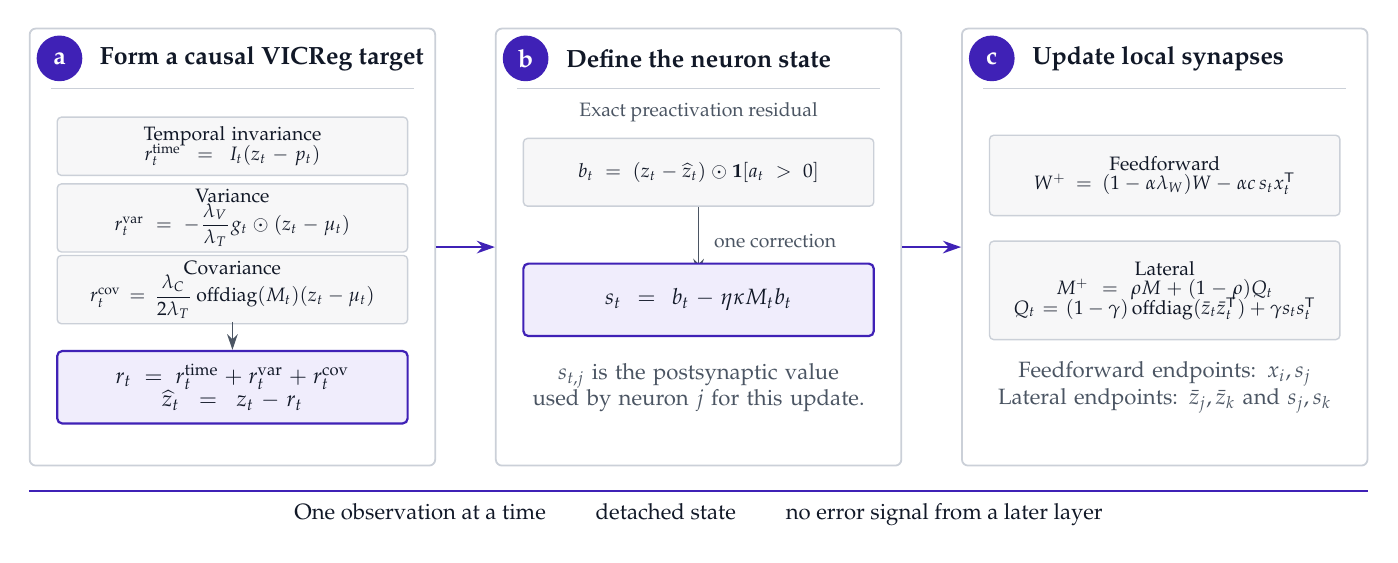
\begin{tikzpicture}[x=1cm,y=1cm]
  \coordinate (A) at (0,0);
  \coordinate (B) at (5.92,0);
  \coordinate (C) at (11.84,0);

  \node[stage] (stage-a) at (A) {};
  \node[stage] (stage-b) at (B) {};
  \node[stage] (stage-c) at (C) {};

  % Identical stage headers establish one reading order and one type system.
  \node[number] at ($(stage-a.north west)+(0.39,-0.39)$) {a};
  \node[anchor=west,font=\small\bfseries,text=AxymInk]
    at ($(stage-a.north west)+(0.78,-0.39)$) {Form a causal VICReg target};

  \node[number] at ($(stage-b.north west)+(0.39,-0.39)$) {b};
  \node[anchor=west,font=\small\bfseries,text=AxymInk]
    at ($(stage-b.north west)+(0.78,-0.39)$) {Define the neuron state};

  \node[number] at ($(stage-c.north west)+(0.39,-0.39)$) {c};
  \node[anchor=west,font=\small\bfseries,text=AxymInk]
    at ($(stage-c.north west)+(0.78,-0.39)$) {Update local synapses};

  \draw[AxymRule,line width=0.55pt]
    ($(stage-a.north west)+(0.28,-0.77)$) --
    ($(stage-a.north east)+(-0.28,-0.77)$);
  \draw[AxymRule,line width=0.55pt]
    ($(stage-b.north west)+(0.28,-0.77)$) --
    ($(stage-b.north east)+(-0.28,-0.77)$);
  \draw[AxymRule,line width=0.55pt]
    ($(stage-c.north west)+(0.28,-0.77)$) --
    ($(stage-c.north east)+(-0.28,-0.77)$);

  % Stage 1: the three terms of the causal VICReg surrogate.
  \node[row] at ($(A)+(0,1.28)$)
    {Temporal invariance\\[-1pt]$r_t^{\mathrm{time}}=I_t(z_t-p_t)$};
  \node[row] at ($(A)+(0,0.37)$)
    {Variance\\[-1pt]
     $r_t^{\mathrm{var}}=-\dfrac{\lambda_V}{\lambda_T}
       g_t\odot(z_t-\mu_t)$};
  \node[row] at ($(A)+(0,-0.54)$)
    {Covariance\\[-1pt]
     $r_t^{\mathrm{cov}}=\dfrac{\lambda_C}{2\lambda_T}
       \operatorname{offdiag}(M_t)(z_t-\mu_t)$};
  \node[result] (target) at ($(A)+(0,-1.78)$)
    {$r_t=r_t^{\mathrm{time}}+r_t^{\mathrm{var}}+r_t^{\mathrm{cov}}$\\[-1pt]
     $\widehat z_t=z_t-r_t$};
  \draw[down] ($(A)+(0,-0.95)$) -- (target.north);

  % Stage 2: exact ReLU residual followed by exactly one correction.
  \node[row,minimum height=0.86cm] (base) at ($(B)+(0,0.95)$)
    {$b_t=(z_t-\widehat z_t)\odot\mathbf 1[a_t>0]$};
  \node[anchor=south,font=\scriptsize,text=AxymMuted]
    at ($(base.north)+(0,0.08)$) {Exact preactivation residual};
  \draw[down] (base.south) -- node[right=2pt,font=\scriptsize,text=AxymMuted]
    {one correction} ($(base.south)+(0,-0.86)$);
  \node[result] (state) at ($(B)+(0,-0.67)$)
    {$s_t=b_t-\eta\kappa M_t b_t$};
  \node[font=\footnotesize,text=AxymMuted,align=center,text width=4.25cm]
    at ($(B)+(0,-1.78)$)
    {$s_{t,j}$ is the postsynaptic value\\
     used by neuron $j$ for this update.};

  % Stage 3: the same postsynaptic factor reaches both synapse types.
  \node[row,minimum height=1.02cm] (ff) at ($(C)+(0,0.91)$)
    {Feedforward\\[-1pt]
     $W^+=(1-\alpha\lambda_W)W-\alpha c\,s_tx_t^{\mathsf T}$};
  \node[row,minimum height=1.25cm] (lat) at ($(C)+(0,-0.55)$)
    {Lateral\\[-1pt]$M^+=\rho M+(1-\rho)Q_t$\\[-1pt]
     $Q_t=(1-\gamma)\operatorname{offdiag}(\bar z_t\bar z_t^{\mathsf T})
       +\gamma s_ts_t^{\mathsf T}$};
  \node[font=\footnotesize,text=AxymMuted,align=center,text width=4.25cm]
    at ($(C)+(0,-1.78)$)
    {Feedforward endpoints: $x_i,s_j$\\
     Lateral endpoints: $\bar z_j,\bar z_k$ and $s_j,s_k$};

  % Short arrows live entirely in equal gutters.
  \draw[next] ($(stage-a.east)+(0,0)$) -- ($(stage-b.west)+(0,0)$);
  \draw[next] ($(stage-b.east)+(0,0)$) -- ($(stage-c.west)+(0,0)$);

  % One footer states why the construction matters.
  \draw[AxymPrimary,line width=0.8pt]
    ($(stage-a.south west)+(0,-0.31)$) --
    ($(stage-c.south east)+(0,-0.31)$);
  \node[anchor=north,font=\footnotesize,text=AxymInk,align=center]
    at ($(B)+(0,-3.13)$)
    {One observation at a time \qquad
     detached state \qquad
     no error signal from a later layer};
\end{tikzpicture}
\end{document}
